\documentclass{article}
\usepackage[T1]{fontenc}
\usepackage[utf8]{inputenc}
\usepackage{lmodern}
\usepackage{amsmath}
\usepackage{sansmath}
\AtBeginDocument{\sansmath}
\renewcommand{\familydefault}{\sfdefault}
\usepackage[paperwidth=19cm,paperheight=14cm,margin=0.4cm]{geometry}
\usepackage{graphicx}
\usepackage{tikz}
\usetikzlibrary{positioning,fit,calc,arrows.meta,backgrounds,decorations.pathreplacing}
\pagestyle{empty}
\setlength{\parindent}{0pt}
\graphicspath{{img/}}

\definecolor{ink}{HTML}{0A0A0A}
\definecolor{muted}{HTML}{6A6A69}
\definecolor{line}{HTML}{BDBDBA}
\definecolor{red}{HTML}{E03A3A}
\definecolor{blue}{HTML}{2E6FE0}
\definecolor{yellow}{HTML}{D9A11A}
\definecolor{green}{HTML}{23A06A}
\definecolor{model}{HTML}{8C8C8A}

\tikzset{
  every picture/.style={font=\sffamily\small, line cap=round, line join=round},
  flecha/.style={-{Stealth[length=2.3mm,width=1.7mm]}, line width=0.7pt, draw=ink},
  grupo/.style={draw=#1, dash pattern=on 3pt off 2pt, line width=0.8pt, rounded corners=2pt, inner sep=6pt},
  titulo/.style={font=\sffamily\small\bfseries, text=#1, anchor=south west, inner sep=1pt},
  foto/.style={inner sep=0pt, outer sep=0pt, draw=ink, line width=0.5pt},
  caja/.style={draw=ink, line width=0.5pt, fill=#1, text=white, font=\sffamily\scriptsize\bfseries,
    text width=3.75cm, minimum height=0.46cm, align=center, inner sep=1.5pt},
  nota/.style={font=\sffamily\scriptsize, text=muted, align=center, inner sep=1pt},
  etapa/.style={font=\sffamily\footnotesize\bfseries, text=ink, align=center, inner sep=1pt},
  paso/.style={draw=ink, line width=0.5pt, fill=#1, text=ink, font=\sffamily\scriptsize, align=center,
    inner sep=3pt, minimum height=0.95cm, text width=2.35cm},
  paso/.default=white,
  grupofondo/.style={draw=#1, line width=0.8pt, fill=#1!6, rounded corners=3pt, inner sep=7pt},
  llave/.style={decorate, decoration={brace, mirror, amplitude=5pt, raise=2pt}, line width=0.7pt, draw=#1},
  llavetexto/.style={font=\sffamily\small\bfseries, text=#1, align=center},
}

\begin{document}
\begin{tikzpicture}

\node[foto] (target) at (0, 0) {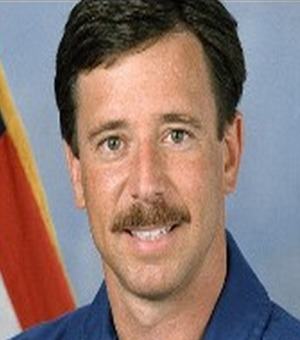
\includegraphics[width=1.85cm]{g2_target.jpg}};
\node[etapa, above=4pt of target] {Imagen objetivo};

\node[paso, text width=2.55cm] (init) at (2.95, 0) {\textbf{Inicialización}\\más gaussianas\\en los bordes:\\$p \propto 0{,}35 + |\nabla I|$};

\node[paso, text width=2.45cm] (render) at (6.25, 1.15) {\textbf{Render}\\$C(x)=\sum_i c_i\,G_i(x)$};
\node[paso, text width=2.45cm] (error) at (9.2, 1.15) {\textbf{Error}\\MSE contra la imagen};
\node[paso, text width=2.45cm] (grad) at (9.2, -1.15) {\textbf{Gradientes}\\analíticos: $\partial q/\partial l_1 = 2u\,d_x$};
\node[paso, text width=2.45cm] (adam) at (6.25, -1.15) {\textbf{Adam}\\escrito a mano;\\$\Sigma^{-1}=LL^\top$};
\draw[flecha] (render) -- (error);
\draw[flecha] (error) -- (grad);
\draw[flecha] (grad) -- (adam);
\draw[flecha] (adam) -- (render);
\node[nota, font=\sffamily\scriptsize\bfseries] at (7.72, 0) {110 a 160\\iteraciones};
\node[grupo=red, fit=(render)(error)(grad)(adam)] (loop) {};
\node[titulo=red] at (loop.north west) {Optimización (sin PyTorch)};

\node[foto] (few) at (12.45, 1.0) {
\includegraphics[width=1.3cm]{g2_pocas.jpg}};
\node[nota, below=1pt of few] (fl) {60};
\node[foto] (many) at (13.9, 1.0) {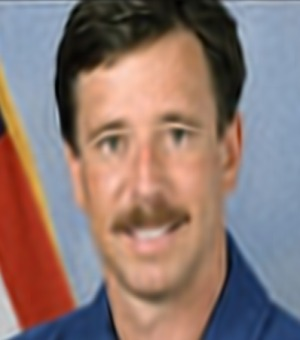
\includegraphics[width=1.3cm]{g2_render.jpg}};
\node[nota, below=1pt of many] (ml) {1500};
\node[foto] (ell) at (13.175, -1.2) {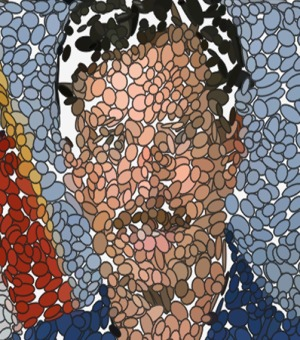
\includegraphics[width=1.3cm]{g2_ellipses.jpg}};
\node[nota, below=1pt of ell] (el) {cada gaussiana};
\node[grupo=green, fit=(few)(many)(ell)(el)(fl)] (out) {};
\node[titulo=green] at (out.north west) {Resultado};

\draw[flecha] (target) -- (init);
\draw[flecha] (init.east) -- (loop.west |- init.east);
\draw[flecha] (loop.east |- 0, 0) -- (out.west |- 0, 0);

\coordinate (base) at ($(out.south) + (0, -0.08)$);
\draw[llave=ink] (init.west |- base) -- (loop.east |- base)
  node[midway, below=9pt, llavetexto=ink] {Implementado por el equipo};
\draw[llave=green] (out.west |- base) -- (out.east |- base)
  node[midway, below=9pt, llavetexto=green] {+8 dB por cada $\times10$};

\end{tikzpicture}
\end{document}
